\documentclass[12pt,a4paper]{article}
\usepackage[T1]{fontenc}
\usepackage[a4paper]{geometry}
\usepackage[portuges,brazilian]{babel}
\usepackage[utf8]{inputenc}
\usepackage{setspace}
\usepackage{libertine}
\usepackage{graphicx}	
\usepackage{ragged2e} 	
\usepackage{hyperref}	

\begin{document} 
\begin{figure}
    \flushright
    
\includegraphics[scale=0.5]{Logo_senai.png}
\end{figure}

\title{Robótica na reabilitação de pessoas com deficiências físicas. - Estratégia}
\author{Jean Paulo Silva\thanks{jean.silva@fbter.org.br SENAI-CIMATEC  CCRoSA- Centro de Competência em Robótica e Sistemas Autônomos.}}
 
 

    \maketitle
    \pagenumbering{arabic}
    \singlespacing

    \section{Estilo dos Slides}
    \begin{itemize}
        \item Fundo branco com detalhes azuis;
        \item Como a maior parte das referências são de artigos e vídeos, trazer gráficos e imagens para os dados estatísticos e gifs animados para os vídeos;
        \item Trazer um máximo de 20 slides em fonte Arial com fonte de no mínimo tamanho 28;
    \end{itemize}
    \begin{figure}[ht]
        \caption{Exemplo de slide}
        \centering
        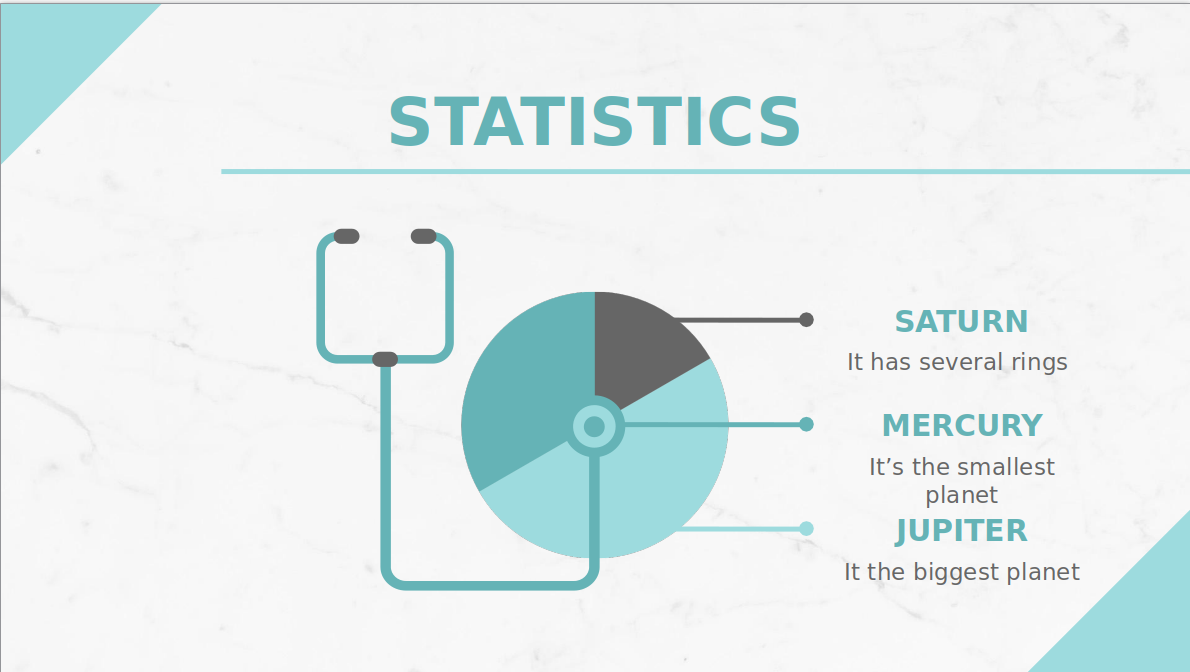
\includegraphics[width=1\linewidth]
        {images/exemplo.png}
        \label{fig:exemplo}
    \end{figure}

    \newpage
    \newpage
    
    \section{Slide - Capa}
    Trazer meu nome, formação e o título da apresentação como capa.

    \section{Slide - História}
    Trazer a história que eu tenho sobre meus familiares e amigos e os medos que eles possuem da amputação e possível dependência.

    \section{Slide - Estimativas}
    Trazer as estimativas de acidentes presentes no meu contexto e como isso pode afetar tanto socialmente quanto emocionalmente uma pessoa.

    \section{Conjunto de Slides Ari Ribeiro}
    Mostrar a história deste caso utilizando gifs animados dos cortes mais relevantes à apresentação.
    Cada slide mostrará a seguinte sequencia de informações:
    \begin{itemize}
        \item Apresentação do caso;
        \item Como ocorreu o problema;
        \item Problema da prótese do SUS;
        \item Solução inicial;
        \item Acompanhamento médico;
    \end{itemize}

    \section{Importância}
    Trazer a importância do acompanhamento médico na reabilitação, independente das tecnologias implementadas.

    \section{Conjunto de Slides UFRN}
    Apresentação das possibilidades de reabilitação e a importância das pesquisas de robótica e automação utilizando a pesquisa da universidade UFRN e a capacidade de baratear tecnologias.

    \section{Conjunto de Slides Les Baugh}
    Seguindo a mesma estrutura do caso Ari Ribeiro, porém dando ênfase nas últimas tecnologias de próteses que possuem funcionalidades e com um acompanhamento médico desde o início.
    \begin{itemize}
        \item Apresentação do caso;
        \item Como ocorreu o problema;
        \item Solução inicial;
        \item Acompanhamento médico;
    \end{itemize}

    \section{Conclusão}
    Ressaltar a importância das pesquisas de robótica na área de saúde para a conclusão do raciocínio. Realizar os devidos agradecimentos e estar disposto a responder as possíveis perguntas.
    3 Perguntas sobre o tema estarão preparadas e entregues à pessoas dos NT caso não hajam dúvidas após a apresentação.



\end{document}